\chapter{Data Model}\label{ch:datamodel}

\figref{fig:datamodel} shows the analysis classes of the data model used by the
application.

\begin{figure}[htb]
	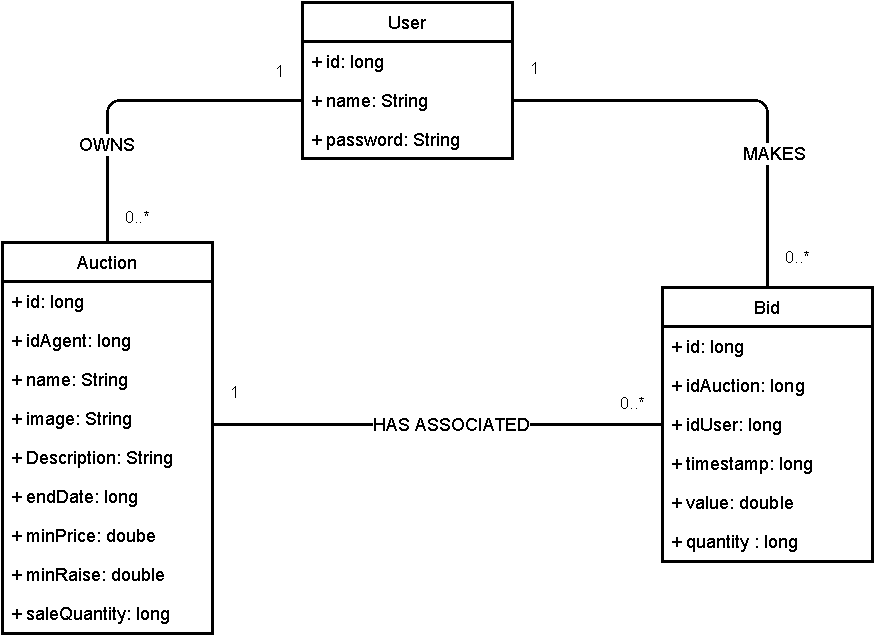
\includegraphics[width=\textwidth]{datamodel}
	\caption{Data model UML diagram (analysis classes).}\label{fig:datamodel}
\end{figure}

\begin{description}
    \item [User]: A registered user.
        \begin{itemize}
            \item \textbf{Id}: unique id of a user;
            \item \textbf{Name}: the username of a user;
            \item \textbf{Password}: the password of a user
        \end{itemize}
    \item [Auction]: An auction of the system
        \begin{itemize}
            \item \textbf{Id}: unique id of an auction;
            \item \textbf{IdAgent}: id of the user that make the auction;
            \item \textbf{Name}: name of the item of the auction;
            \item \textbf{Image}: image of the items of the auction;
            \item \textbf{Description}: description of the items of the auction;
            \item \textbf{EndDate}: the date and time when the auctions ends;
            \item \textbf{MinPrice}: starting price for each item of the bid;
            \item \textbf{MinRaise}: minimum raise for each new bid;
            \item \textbf{SaleQuantity}: number of items to sell
        \end{itemize}
    \item [Bid]: A bid for an auction made by a user
        \begin{itemize}
            \item \textbf{Id}: unique id of a bid;
            \item \textbf{IdAuction}: id of the auction;
            \item \textbf{IdUser}: id of the user that made the bid;
            \item \textbf{Timestamp}: timestamp the bid was made;
            \item \textbf{BidValue}: value of the bid for single item;
            \item \textbf{Quantity}: number of items you want to buy
        \end{itemize}
\end{description}
